\documentclass[12pt]{article}

%% preamble: Keep it clean; only include those you need

% if the below packages cannot be installed automatically, you can 
% download the required .sty files from CTAN and place them in the
% same location as the .tex file (or upload to overleaf in same
% location (folder) in overleaf

\usepackage{amsmath}
\usepackage[margin = 1in]{geometry}
\usepackage{graphicx}
\usepackage{booktabs}
\usepackage{natbib}

\usepackage{lineno}  % use these two lines to include line numbers
\linenumbers

\usepackage{setspace} % for doublespacing
\doublespacing


% highlighting hyper links
\usepackage[colorlinks=true, citecolor=blue]{hyperref}


\usepackage{color}
\newcommand{\blue}{\color{blue}} 
% when you make your edits in response to review/instructor comments, 
% you can indicate changes in color

%% meta data

\title{Paradoxical Coastal Property Value Resilience Amid Climate Risks}
\author{Jack Bienvenue\\
  Department of Statistics\\
  University of Connecticut
}

\begin{document}
\maketitle

\begin{abstract}

In spite of dramatically intensifying climate risk factors in the coastal United States, real property valuations appear unharmed, with appreciation even appearing to outpace appreciation experienced by inland properties. In this paper, a novel, open-data method is proposed for seeking evidence for whether coastal property valuations are rising at a rate surpassing inland properties. The analysis in this paper seeks to independently evaluate the finding in the literature that coastal property values have maintained parity in terms of holding value in the face of major climate risks. Despite the past, current, and foreseeable accentuation of climatological risks like sea level rise and intensified storm events, this paper finds no evidence to suggest that coastal property valuations have experienced rates of change unlike those of their inland peers. 

\noindent\textbf{Keywords}: Real Estate, Climate Change, Real Property Valuation, Zillow, Open Data, Sea Level Rise
\end{abstract}


\section{Introduction}
\label{sec:intro}

Climate related risks to real property are growing as anthropogenic climate change accentuates storm events and contributes to sea-level rise (SLR) \citep{griggs2021coastal}. Many regions of the United States have experienced the impacts of intensified storm events, SLR, and other climate change heightened, destructive weather anomalies such as coastal wildfires \citep{reed2022attribution, swain2025increasing}. With 40\% of Americans residing in coastal counties, coastal real property accounts for much of the housing stock in the United States \citep{EPA2025}. The coastal United States is central to economic and human activity in the nation and the costs incurred by individuals and government entities due to weather and climate challenges is immense \citep{reed2022attribution}. Coastal real property is exposed unproportionately to storm and SLR risks in comparison to inland peers \citep{clayton2021climate}. Property damage or destruction risks, and accompanying safety risks, would be expected to affect coastal real estate valuations negatively. However, in past years, coastal property values have been observed to continue to rise. 

A large variety of factors influence real estate valuations. In an efficient housing market, one could expect all factors to combine to determine the fair valuation of a home \citep{maier2009real}. Some in the scientific community believe that climatological risks are under priced in real estate valuations---that is, that because market participants may be underestimating relatively new, but growing, risks to a home caused by climate change effects like intensified storms and sea level rise \citep{McNamara2024}. 

Underpricing of such risks could have devastating consequences. Home equity is an important asset for homeowners. Home destruction or damage due to climate change could seriously impact the prosperity of many residents of coastal areas \citep{fussell2014homeownership}. While coastal real estate is colloquially synonymous with lavish, expensive properties, in actuality there is a great diversity of coastal county residents, including many low and middle income Americans. If the true extent of coastal risk is not priced into real estate valuations, when these risks are reflected in prices, American homeowners across the socioeconomic spectrum may experience significant losses \citep{McNamara2024}.

The aforementioned potential loss in home values through recognition of coastal risks, if they are not presently priced in, presents the possibility of a major depreciation event for coastal property that could disrupt real estate markets at a much broader scale. This analysis will determine whether valuation movements in coastal real estate markets are significantly different from non-coastal real estate valuation movements. Non-coastal properties are assumed to have less real and perceived climate change risk exposure from intensified storms and sea level rise for comparison in this analysis. 

This analysis will build a method for independently verifying or the assertion made in \citet{McNamara2024} that coastal real estate prices remain steady or on the rise as compared to inland peers.

\section{Data Description}
\label{sec:data}

Data for this analysis come from a variety of reputable entities. The primary dataset containing real estate valuations originates from the most popular real estate platform Zillow. This data can be accessed freely to individuals via NASDAQ Data Link. The entirety of the available dataset was downloaded for this analysis. This dataset has a size of about 5.5 GB and contains hundreds of thousands of entries relating to dozens of indicators. The vast majority of the data report listed valuations of real property, each with its date and region identifier listed. An indicator identifier is also provided to provide context to the property, like whether it is a single-family home, condominium, one bedroom home, two bedroom home, etc. Table \ref{tab:zillowmain} below provides a very small sample of the data. The indicator identifier ``ZSFH" denotes that these properties are listed as single-family homes.

\begin{table}[h]
  \caption{This table includes sample data from the Zillow dataset.}
  \label{tab:zillowmain}
\centering
\begin{tabular}{lrrr}
  \toprule
  indicator\_id & region\_id & date & value \\
  \midrule
  ZSFH & 74221 & 7/31/96 & 101485 \\
  ZSFH & 274631 & 11/30/96 & 73820 \\
  ZSFH & 41236 & 11/30/96 & 102436 \\
  ZSFH & 5967 & 10/31/96 & 171608 \\
  \bottomrule
\end{tabular}
\end{table}

Indicators excluded from this analysis are those which do not relate to real estate valuations. These include home-selling temporal variables like time spent listed on the market and the share of properties which have had price cuts of the housing stock for sale in a region. Such indicators are irrelevant for the purpose of this analysis, but may be of interest in future work.

This primary Zillow dataset is accompanied by two auxiliary tables. The first is the indicator table, which provides a key for interpretation of the indicator abbreviations. The second table provides a key the region identifiers, providing the corresponding name of the region. An excerpt of this data is shown below in Table \ref{tab:region_data}:

\begin{table}[h]
  \caption{This table demonstrates regional encoding data.}
  \label{tab:region_data}
\centering
\begin{tabular}{rll}
  \toprule
  region\_id & region\_type & region \\
  \midrule
  394415 & metro & Bridgeport, CT \\
  2288 & county & Franklin County;OH;Columbus, OH \\
  394653 & metro & Greenville, SC \\
  394312 & metro & Albuquerque, NM \\
  \bottomrule
\end{tabular}
\end{table}

As seen above, there is variety in the formatting of the region column. To spatially localize the properties to their coastal or non-coastal designation, a convention was devised for handling region names which reference multiple places. This involved stripping the information from the first place mentioned and geocoding---extracting latitude and longitude data---that place as the location of the home. While extracting the first place name from separated items of list-formatted regions is arbitrary, it provides consistency and often provides a county name. The utility of this will be explained in Section \ref{sec:meth}.

Data are anonymized in the Zillow dataset. Exact location details of properties are hidden to protect market participants including homeowners and sellers. This lack of granularity necessarily means that the spatial precision of the analysis is limited by the provided information. The geocoding method proposed in this paper seeks to use a commonsense method for approximating locations of properties at a sufficient spatial resolution for assignment of properties to coastal and non-coastal areas. The geocoding process is further explained in Section \ref{sec:meth}.

The Zillow dataset contains home valuation data from the year 1996 to the year 2024. It is regularly updated, providing the possibility for the analysis in this paper to be revisited in the future. Upon first inspection of the data, it becomes clear that there could be reason to suspect discrepancies between coastal and non-coastal valuations, as shown in Table \ref{tab:descriptive_statistics}.

\begin{table}[h]
  \caption{Descriptive Statistics for Coastal and Non-Coastal Data.}
  \label{tab:descriptive_statistics}
  \centering
  \begin{tabular}{rll}
    \toprule
    \textbf{Statistic} & \textbf{Non-coastal} & \textbf{Coastal} \\
    \midrule
    Count & 78796.0 & 24763.0 \\
    Mean (\$) & 194844.09 & 351458.97 \\
    St. Dev. (\$) & 189868.28 & 430689.37 \\
    Min (\$) & 5523.16 & 11956.22 \\
    25\% Quartile (\$) & 93229.75 & 135919.79 \\
    Median (\$) & 146261.66 & 230891.10 \\
    75\% Quartile (\$) & 234274.50 & 411104.50 \\
    Max (\$) & 10890610 & 10580380 \\
    \bottomrule
  \end{tabular}
\end{table}

Principles of data ethics are observed in the use of this data. As mentioned previously, data are anonymous and reflect reporting from a reputable entity in the field. Further, sub-sampling techniques (explained in Section \ref{sec:meth}) are done randomly. All random processes pertaining to the data were performed in reproducible ways. This analysis does not disseminate information about individuals directly or indirectly, and does not source its data from dubious sources. Transparency surrounding data is prioritized throughout this paper.

Outside of the primary Zillow data, necessary for this analysis is a shapefile of the nation's counties. This was gathered from the United States Census Bureau \citep{USCensusCountyShapefile2025}. Coastal counties were selected through manual inspection and selection. Coastal counties include all United States counties abutting the Atlantic and Pacific Oceans, as well as the Great Lakes. Counties abutting the Great Lakes were included as they reflect sensitivity to climate change which are driven by changes in the bodies of water. \cite{theuerkauf2021rapid}

\section{Methods}
\label{sec:meth}

This section provides information on the intricacies of final data preparation and the design of the statistical tests employed.

\subsection{Subsampling Technique}

The Zillow dataset contains hundreds of thousands of entries, a scale too impractical for local processing. Instead of using the entirety of the data for the analysis, this paper instead utilizes a randomized selection of entries in the table to reduce computational time. 

There are two ways in which balance is important in the dataset in this analysis---the first being temporal balance, having adequate representation of data over time in the dataset, and the second being spatial balance, having adequate representation of data in both the coastal and non-coastal subsets. 

This paper does not control for coastal and non-coastal balance by design. It is assumed that, because the population of the United States falls approximately half inside and half outside of coastal counties, that this balance should emerge organically with adequate sample size. In reality, the subsample included approximately 25\% coastal properties. Because of cloud computing costs and because there were still approximately 25,000 coastal entries, balancing this proportion was not pursued for this project.

\begin{figure}[h]
    \centering
    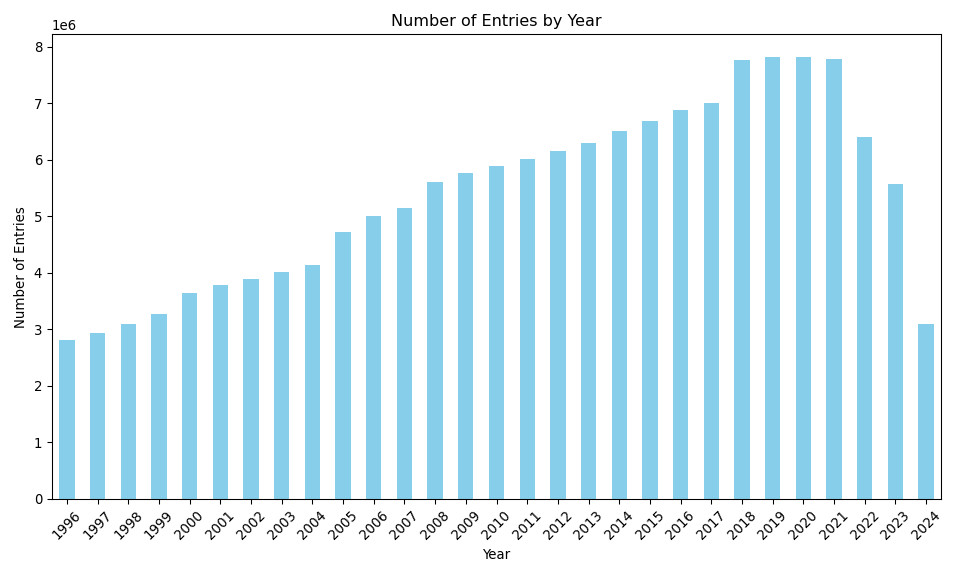
\includegraphics[width=0.9\textwidth]{figures/annual_distribution_of_data.png}
    \caption{Count of entries by year in complete Zillow dataset.}
    \label{fig:annual_distribution_of_entries}
\end{figure}

On the other hand, as displayed in Figure \ref{fig:annual_distribution_of_entries} on the following page, the distribution of entries in the dataset varies widely enough to justify control in our randomized selection. This analysis seeks to evaluate changes over time, so temporal sparsity in data due to random sampling is not an acceptable outcome. Data are sampled randomly within years, but the overall count of data points selected from individual years is fixed at $\frac{\text{total sample size}}{28}$, with $28$ representing the number of years between 1996 and 2024.

Random sampling with large subsample size ($n = 100000$) is used in this analysis. While other subsampling methods have been proposed in the field os statistics for optimizing certain objectives, the very large subsample size ensures that results from the subsample will be consistent to the population to a reasonable degree. 

\subsection{Coastal Designation Scheme}

Analyzing the Zillow dataset necessitates the development of a method for sorting entries into coastal and non-coastal properties, a designation which is not explicitly listed in the source data. 

In addition, Zillow's unique region identification codes exempt the possibility of simple sorting techniques like matching to counties directly, matching to counties through zip codes, or other direct means.

Instead, a geocoding process is required in order to match place names retrieved from matching region identifiers to the regions table (excerpt of this table available in Table \ref{tab:region_data}). Google's Geocoding API was selected as the geocoding tool for this analysis.

Once latitude and longitude values were retrieved from the geocoding process, these points were tested to see whether they fell within the bounds of the coastal county shapefile and designated in binary fashion for whether they were coastal or not.

In Section \ref{sec:data}, references were made to the validity of the spatial matching scheme, especially in regards to multiple-named regions. This method supposes that multiple-named regions have individual place names which represent places close enough together to correctly designate the coastal indicator. In addition, since most first named places on multiple-named regions are county named, the geocoding API generally choose a central latitude/longitude point in the county to represent the county as a place, meaning that when the point is intersected with coastal counties, if it is a coastal county, there should be no issue to the success of the method. 

\subsection{Statistical Testing}

To evaluate whether or not there is evidence to suggest that coastal property valuations are rising unproportionately compared to valuations of the inland property stock, this paper proposes a multiple comparison testing method to test the following hypothesis:

$H_0$: \emph{The difference in the average monthly rate of change of home valuations between coastal and non-coastal counties is zero.}

\textbf{$H_1$}: \emph{The difference in the average monthly rate of change of valuations between coastal and non-coastal counties is not zero.}

This test was implemented using a one-sample t-test. The confidence level for the test was set to $\alpha = 0.05$. The results of the test are shown in Table \ref{tab:test_results} below:

\begin{table}[ht]
\centering
\caption{Outcomes of Test}
\label{tab:test_results}
\begin{tabular}{lr}
\hline
& \textbf{Value} \\
\hline
T-statistic        & 0.2355 \\
P-value            & 0.8139  \\
Sample size n      & 331 \\
\hline
\end{tabular}
\end{table}

\section{Results}
\label{sec:resu}

This analysis finds that there is no statistical evidence suggesting that there is no discrepancy between the average monthly changes in coastal and non-coastal real estate valuations. 

Suggestive of this result is Figure \ref{fig:histogram_of_difference}, the histogram of differences in monthly changes in average real estate valuations for coastal and non coastal properties. This histogram relays the image of an approximately normally distribution of change differences about zero. This result independently verifies the same conclusion made in \citet{McNamara2024}. The selected method represents a relatively simplistic method of testing the relationship between coastal and non-coastal average valuations, demonstrating consistency with literature results in a parsimonious fashion while also opening possibilities for more sophisticated testing methods in the future.

\begin{figure}[h]
    \centering
    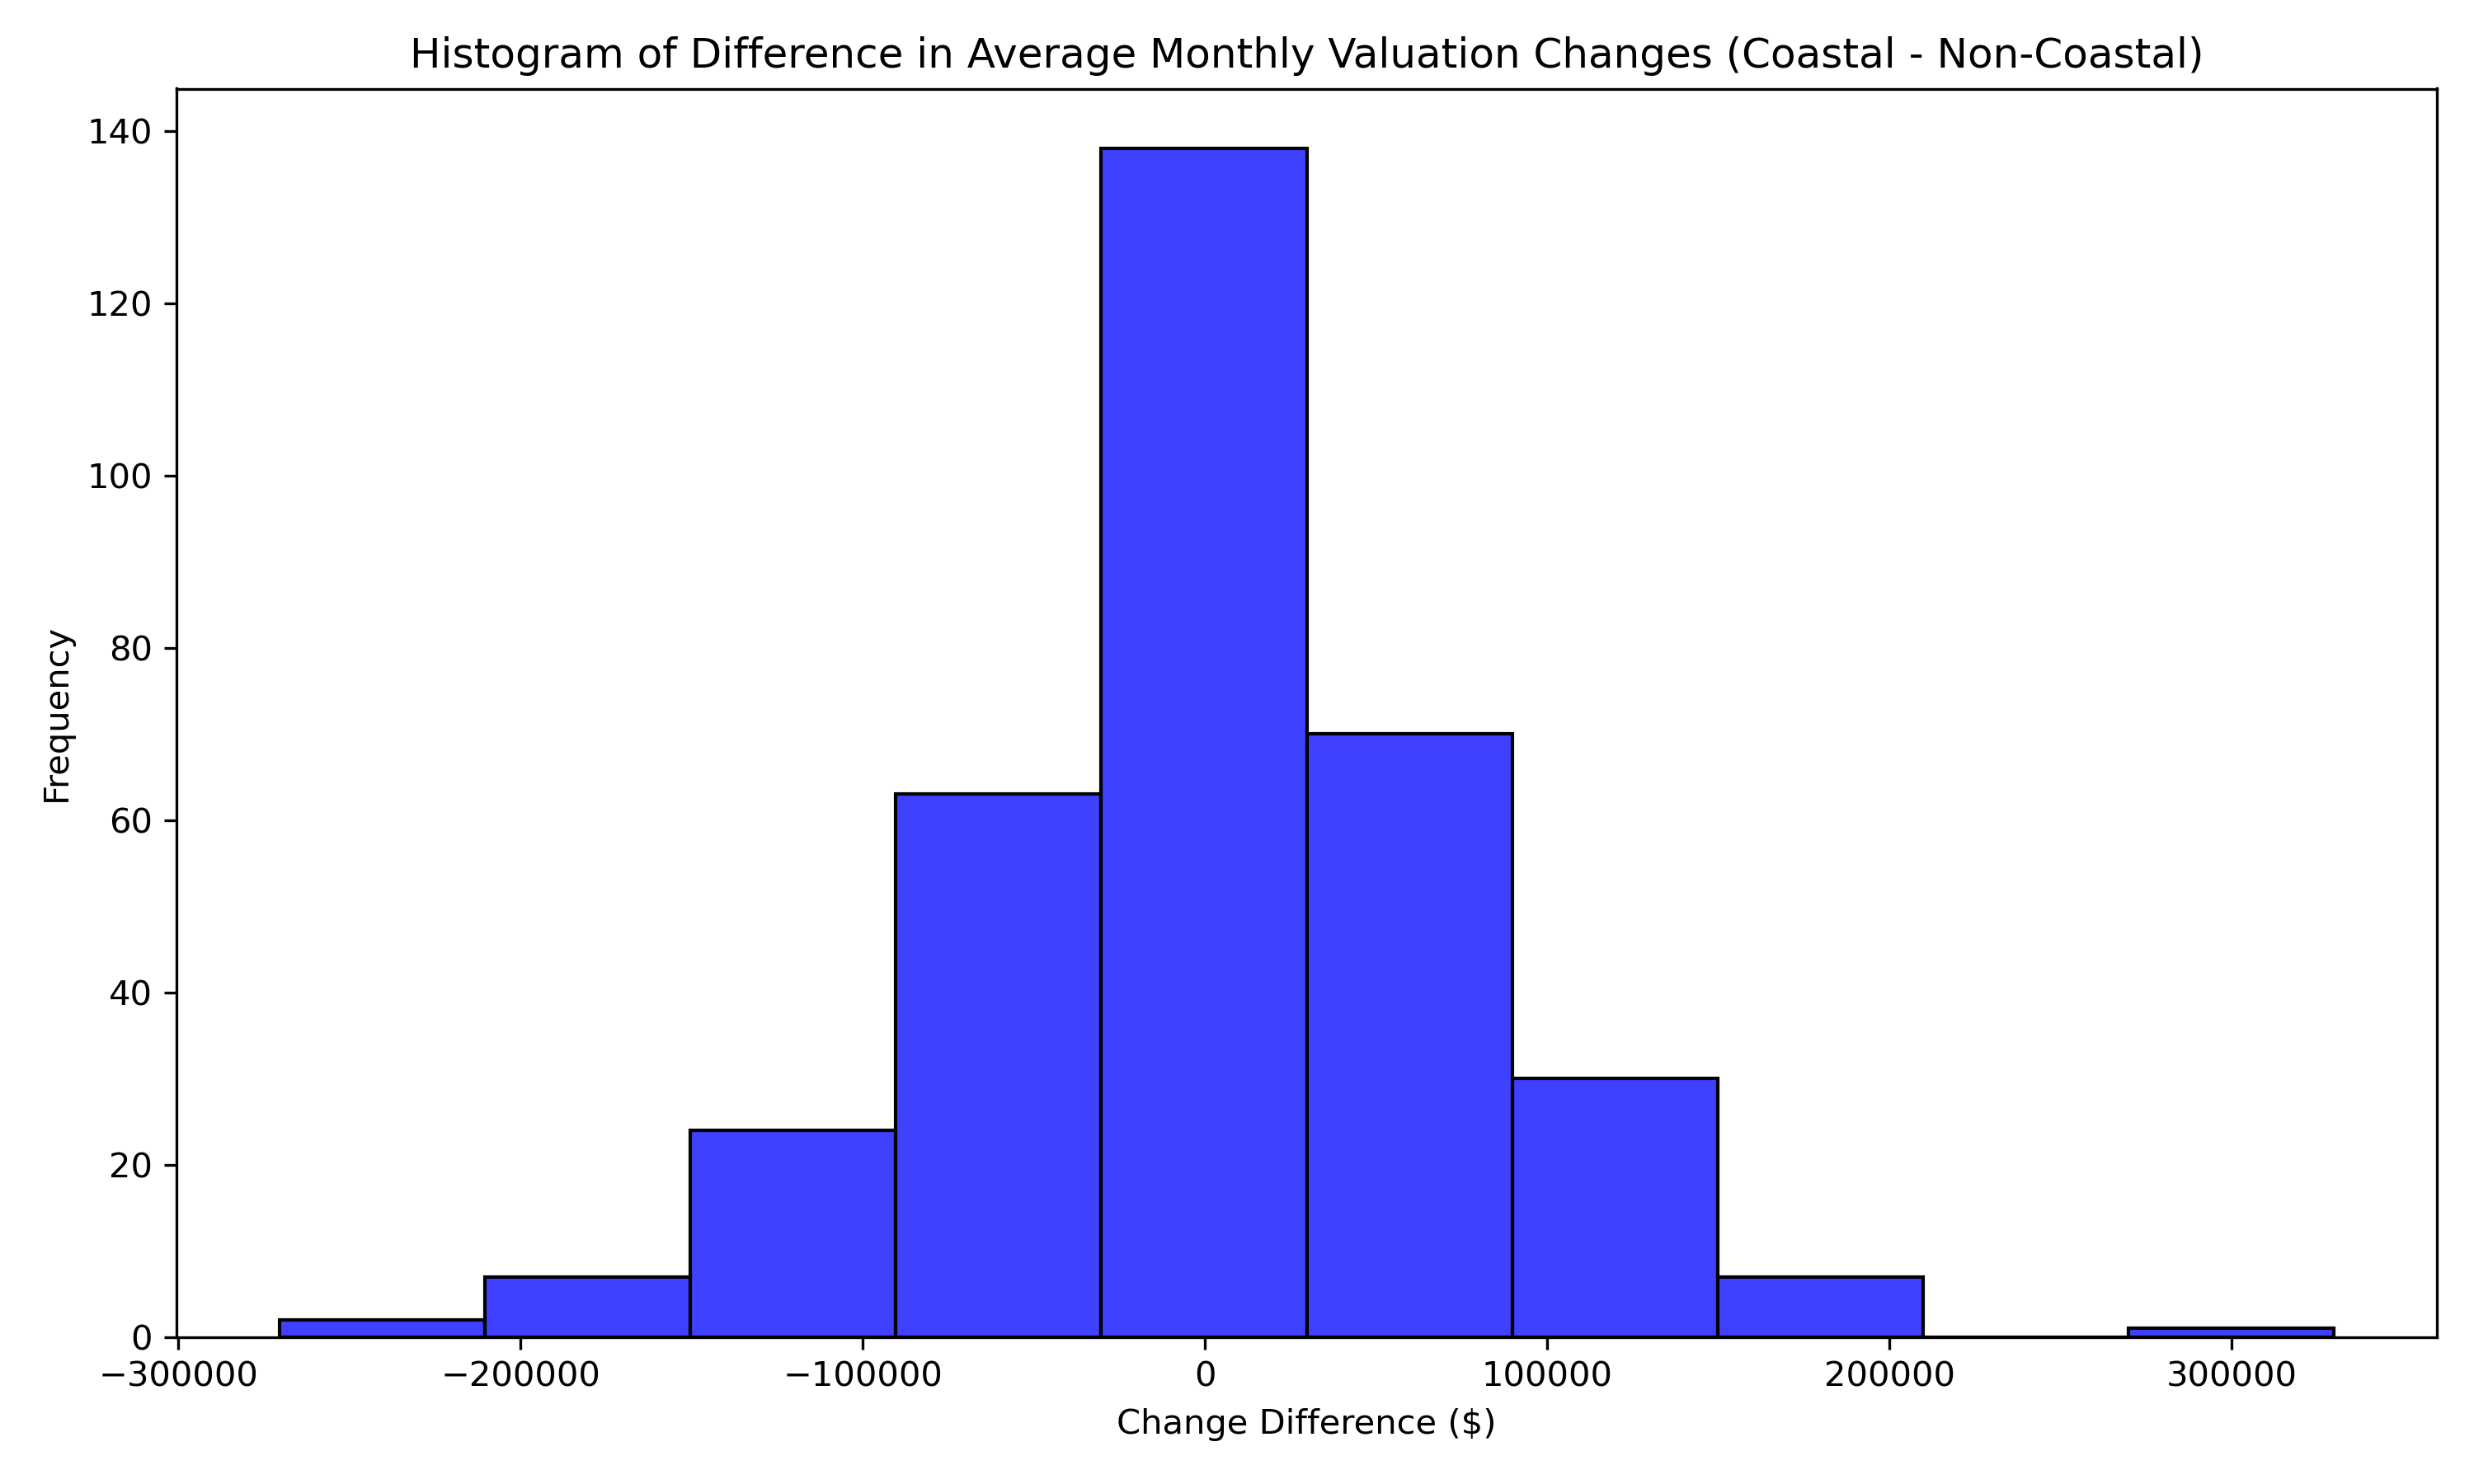
\includegraphics[width=0.75\textwidth]{figures/histogram_of_change_differnces.png}
    \caption{Histogram Representing the Distribution of Monthly Differences in the Change of Average Coastal and Non-Coastal Property Valuations from 1996 to 2024}
    \label{fig:histogram_of_difference}
\end{figure}

\section{Discussion}
\label{sec:disc}

The independent verification in this paper of the finding in \citet{McNamara2024} presents further cause for concern for future valuations in coastal real estate in relation to climatic risks. Figures \ref{fig:monthly_time_series_valuations} and \ref{fig:annual_time_series_valuations} demonstrate the ambiguity in trends which necessitated statistical evaluation to decipher.  

\begin{figure}[h]
    \centering
    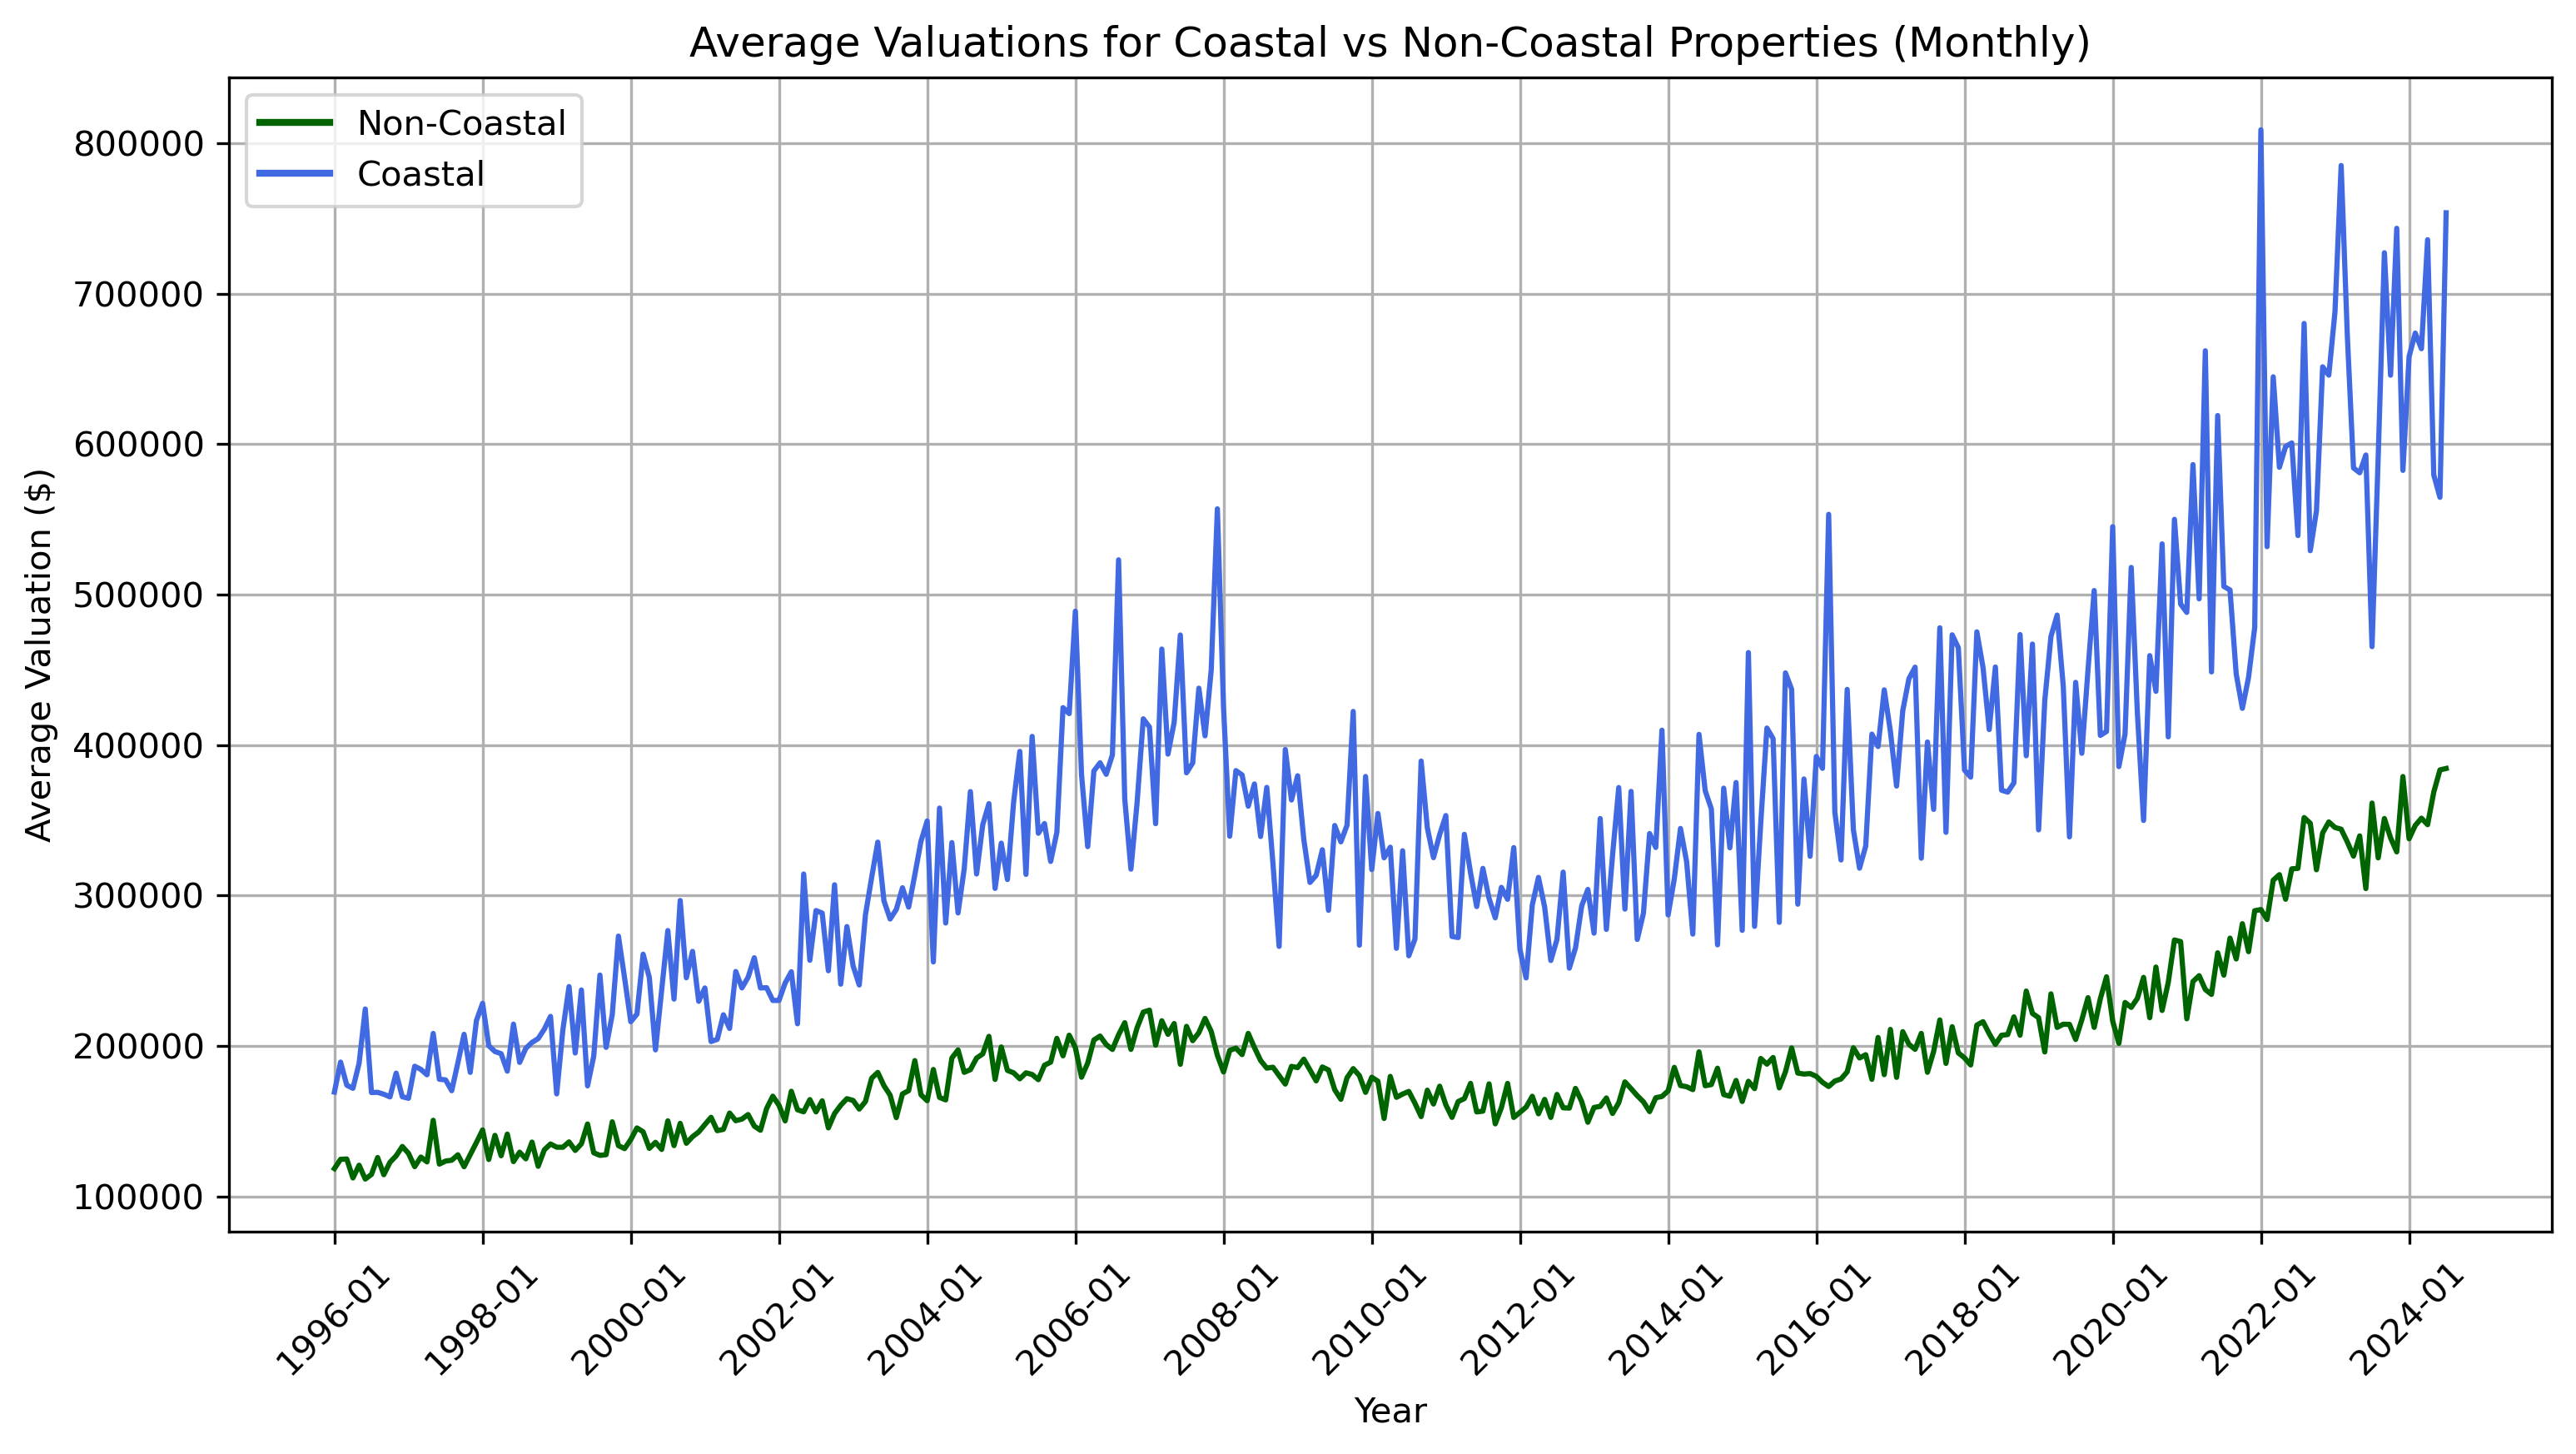
\includegraphics[width=0.8\textwidth]{figures/coastal_vs_non_coastal_monthly.png}
    \caption{Monthly Time Series of Average Coastal and Non-Coastal Property Valuations}
    \label{fig:monthly_time_series_valuations}
\end{figure}

\begin{figure}[h]
    \centering
    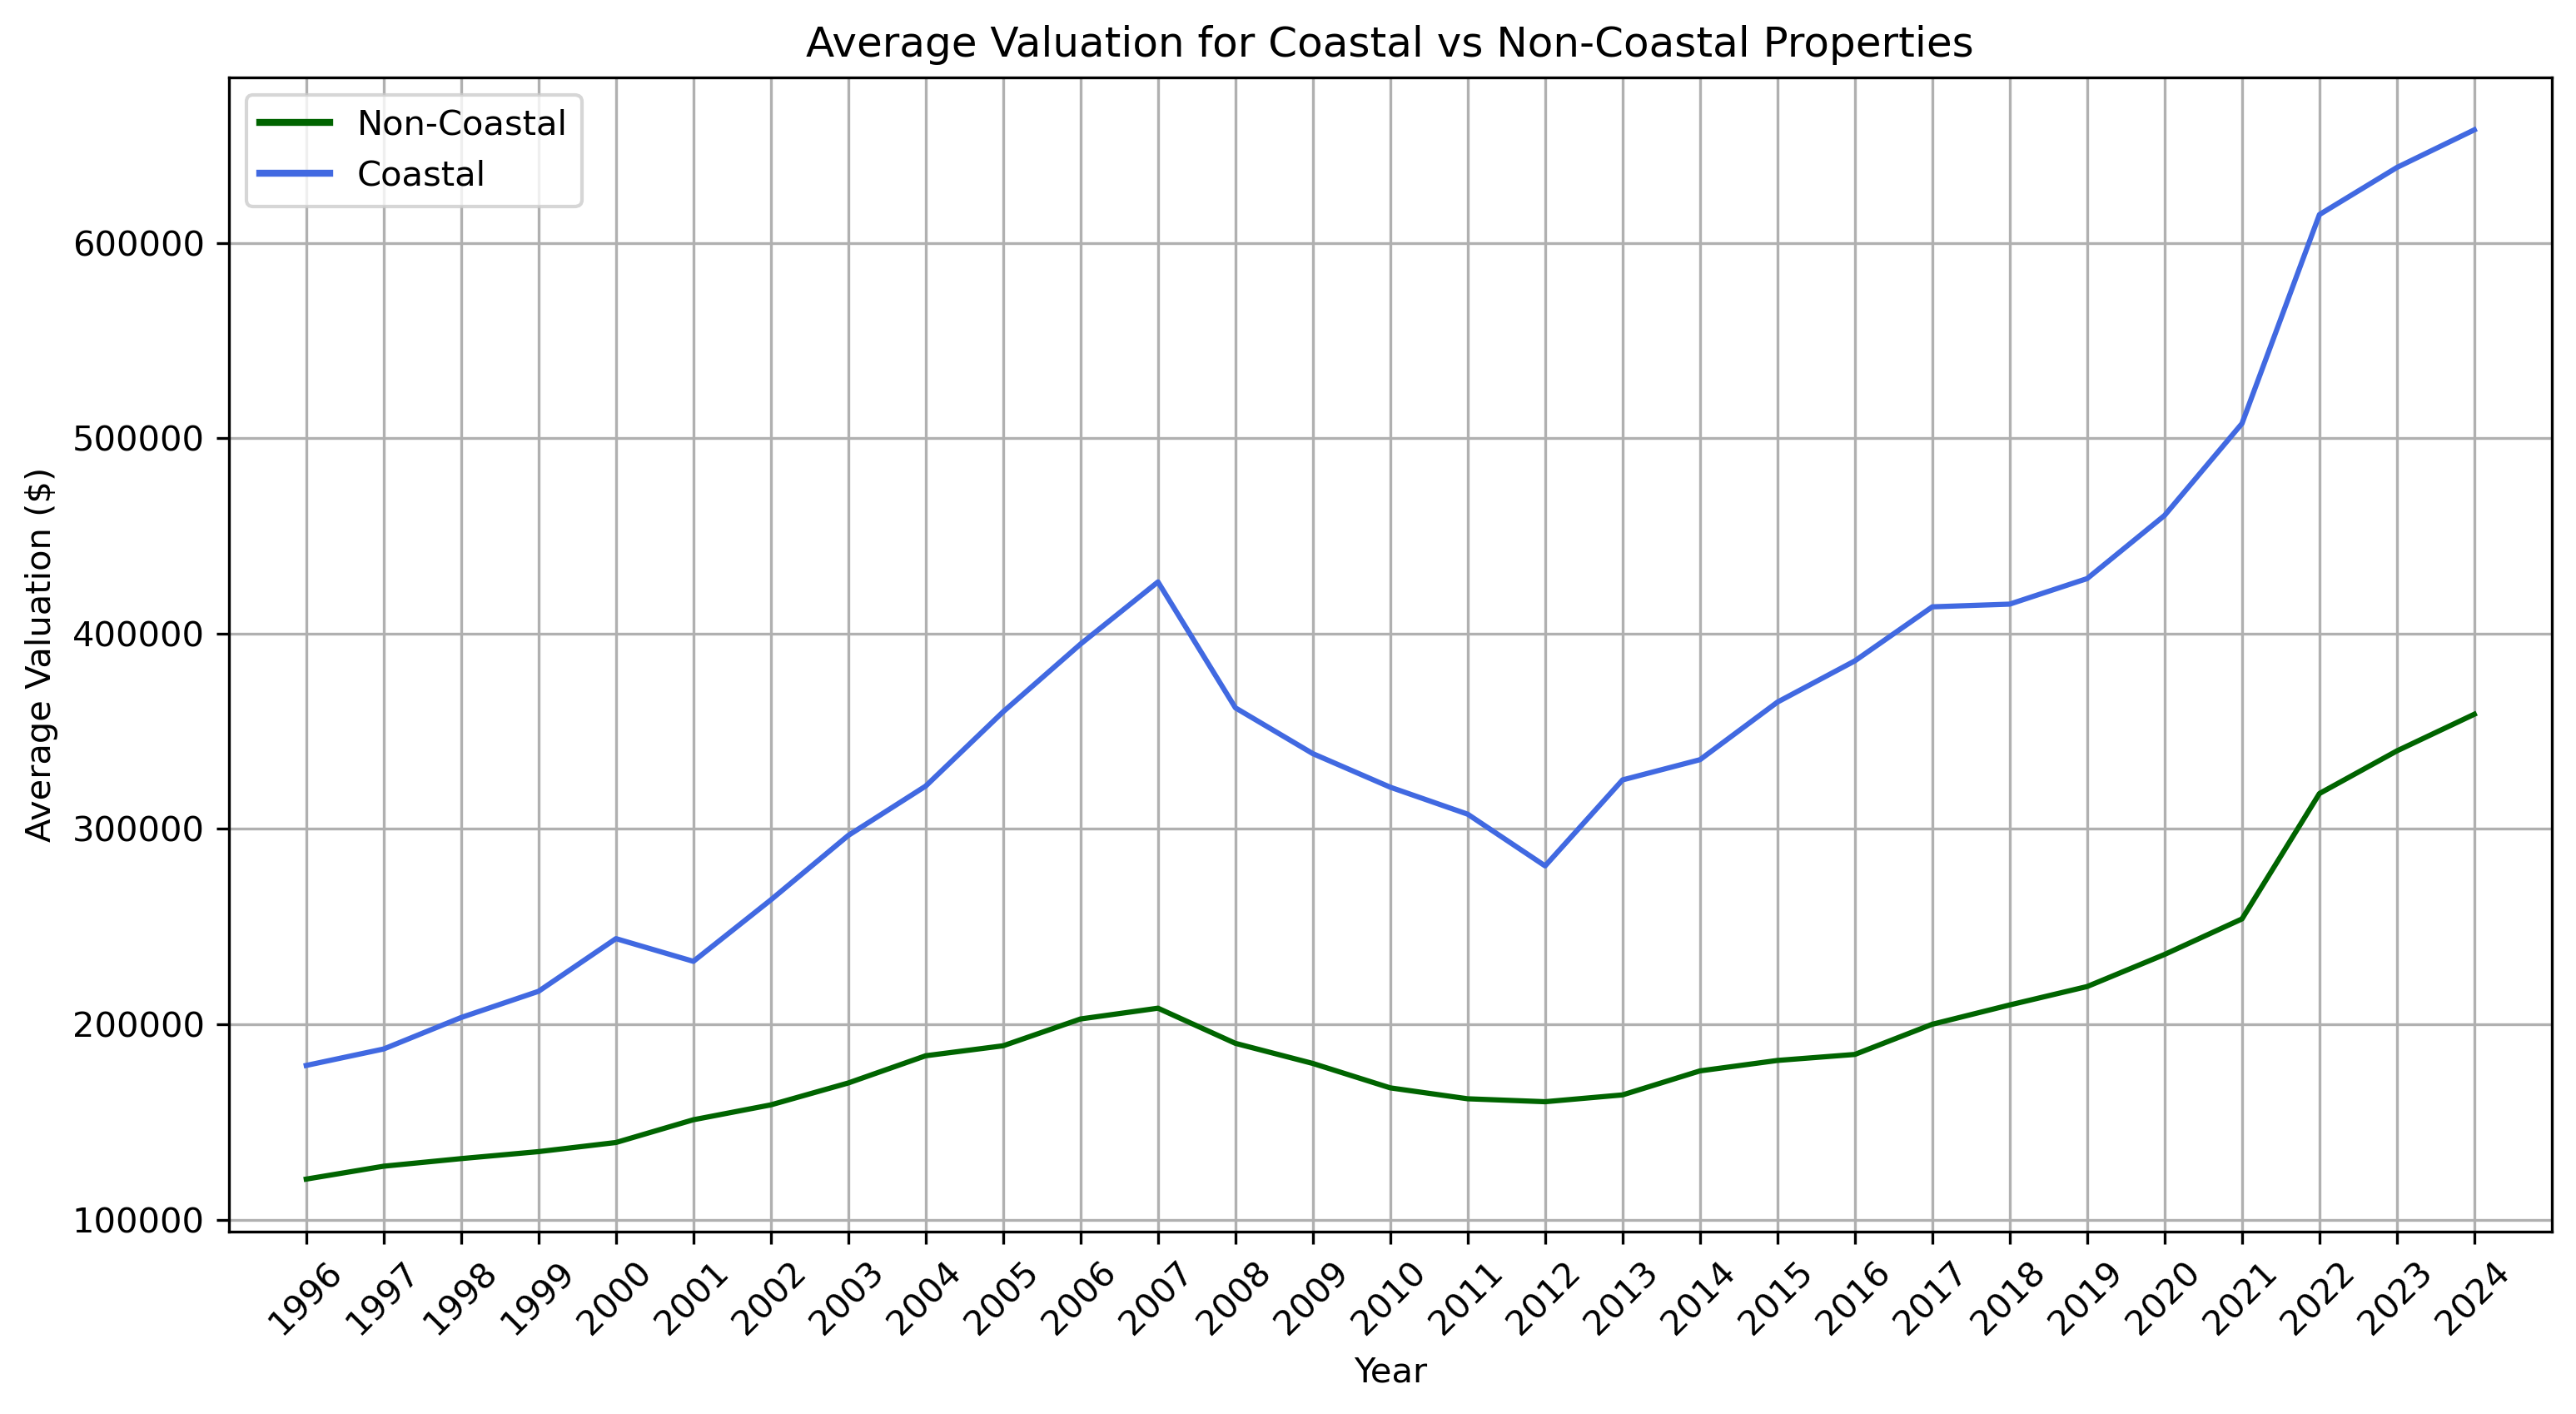
\includegraphics[width=0.8\textwidth]{figures/annual_avg_chart.png}
    \caption{Annual Time Series of Average Coastal and Non-Coastal Property Valuations}
    \label{fig:annual_time_series_valuations}
\end{figure}

\subsection{Topics to Inquire}

A variety of research questions stem from this analysis and are made possible by the construction of the high-quality, large, and spatiotemporally spanning dataset created for this paper. One may wonder if areas which have been affected in strong negative ways by SLR and intensified storms have experience transitory or long lasting home valuations effects compared to the set of inland properties or similar risk level coastal peer counties which did not experience extreme damages from climatic trends. Special interest can be taken also to evaluate spatial differences in valuations between coastal communities with different climatic risk levels, controlling for local real estate valuation variables. Temporal division of data may also yield interesting results as climate change effects have worsened over the period of observation, and perceived and real risks have been on the rise through this period. 

\section*{Supplemental Materials}

All code and data used in this manuscript are available at \url{https://github.com/jackbienvenue/coastal_real_estate_pricing}.

%\section*{Acknowledgements} %optional

\newpage
\bibliography{bibliography/refs.bib}
\bibliographystyle{bibliography/asa.bst}


%\section*{Appendix} %optional


\end{document}